\documentclass[12pt]{article}
	\usepackage[danish]{babel}
	\usepackage{tabularx}
	\usepackage{varwidth}
	\usepackage{array}
    \usepackage[margin=1in]{geometry}
    \usepackage{amsmath}
    \usepackage[utf8]{inputenc}
    \usepackage{graphicx}
    \usepackage{fancyhdr}
    \usepackage{lastpage}
    \usepackage[T1]{fontenc}
    \usepackage{amssymb}
    \usepackage{listings}
    \usepackage{minted}
    \usepackage[colorinlistoftodos]{todonotes}
    \usepackage{wrapfig}
    \usepackage{subcaption}
    \usepackage{hyperref}
    \usepackage{todonotes}
    \usepackage[final]{pdfpages}
    \usepackage{parskip}
    \usepackage{float}
    \usepackage{adjustbox}
    \usepackage{colortbl}
    \usepackage{color}
    \definecolor{Gray}{gray}{0.8}
    \definecolor{LightGray}{gray}{0.9}
    \definecolor{WhiteGray}{gray}{0.95}
    
    \pagestyle{fancy}

    \title{Diabetes og Min Sundhedsplatform - Dybdeanalyse}
    \author{Casper Bresdahl whs715\\ Torben Olai Milhøj vrw704\\ Sarah Willumsen zql291\\ Mads Rosenlund Jensen lfh632\\}
    \date{}
    \begin{document}
        \maketitle
        \thispagestyle{empty}
        \cfoot{Page \thepage ~of \pageref{LastPage}}
        %Af en eller anden grund stod der INDHOLD i sidehovedet, disse tre linjer fjerner dette
        \chead{}
        \lhead{}
        \rhead{}
        %Fjerner linjen i sidehovedet
        \renewcommand{\headrulewidth}{0pt}

        \pagestyle{empty}
        {
        	\renewcommand{\thispagestyle}[1]{}
        	\tableofcontents
        }
        \clearpage
        \pagestyle{fancy}
        \newpage
        \setcounter{page}{1}
        	\section{Forberedelses fasen}
I forberedelses fasen begyndte vi vores projektarbejde med selv at undersøge hvad diabetes er, og hvad det ville sige at leve med diabetes. Vi begyndte derefter at kigge på hvilke funktioner som min sundhedsplatform havde og hvilke siden manglede, som vi kunne forestille os ville styrke den. Vi kom frem til fire ideer - receptfornyelse, læring og videnscenter, socialt samlingssted og en forberedelse af siden til fremtidens teknologi. Gennem et interview og en spørgeskema undersøgelse kom vi frem til at siden kunne forbedres ved at samle funktioner fra andre af sundhedsvæsenets sider, såsom receptfornyelse, og gøre dem tilgængelige på min sundhedsplatform. Ligeledes fandt vi også frem til at brugerne af siden ofte ikke finder frem til den information de søger, og der kunne derfor også samles mere information omkring diabetes på siden.\\
Nøgleordene for at projektet kan lykkes er brugervenlighed, tilgængelighed og udbredelse af kendskab til siden. Vi fandt at mange af vores adspurgte diabetikere ikke kendte til siden, og dem som gjorde var i mange forskellige aldre. Det er derfor vigtigt for projektet at alle kan benytte de funktioner som vil kunne findes på siden, og at brugervenligheden derfor i høj grad er i fokus.\\
Fra vores strategianalyse fandt vi at det er vigtigt med sikre og intuitive løsninger som brugeren selv kan benytte. Der er behov for et samlet system således at brugeren selv kan finde al den nødvendige information. Samtidigt skal løsningerne være afprøvede og testede i drift, og de skal kunne udvides i fremtiden.
\begin{figure}[H]
	\centering
	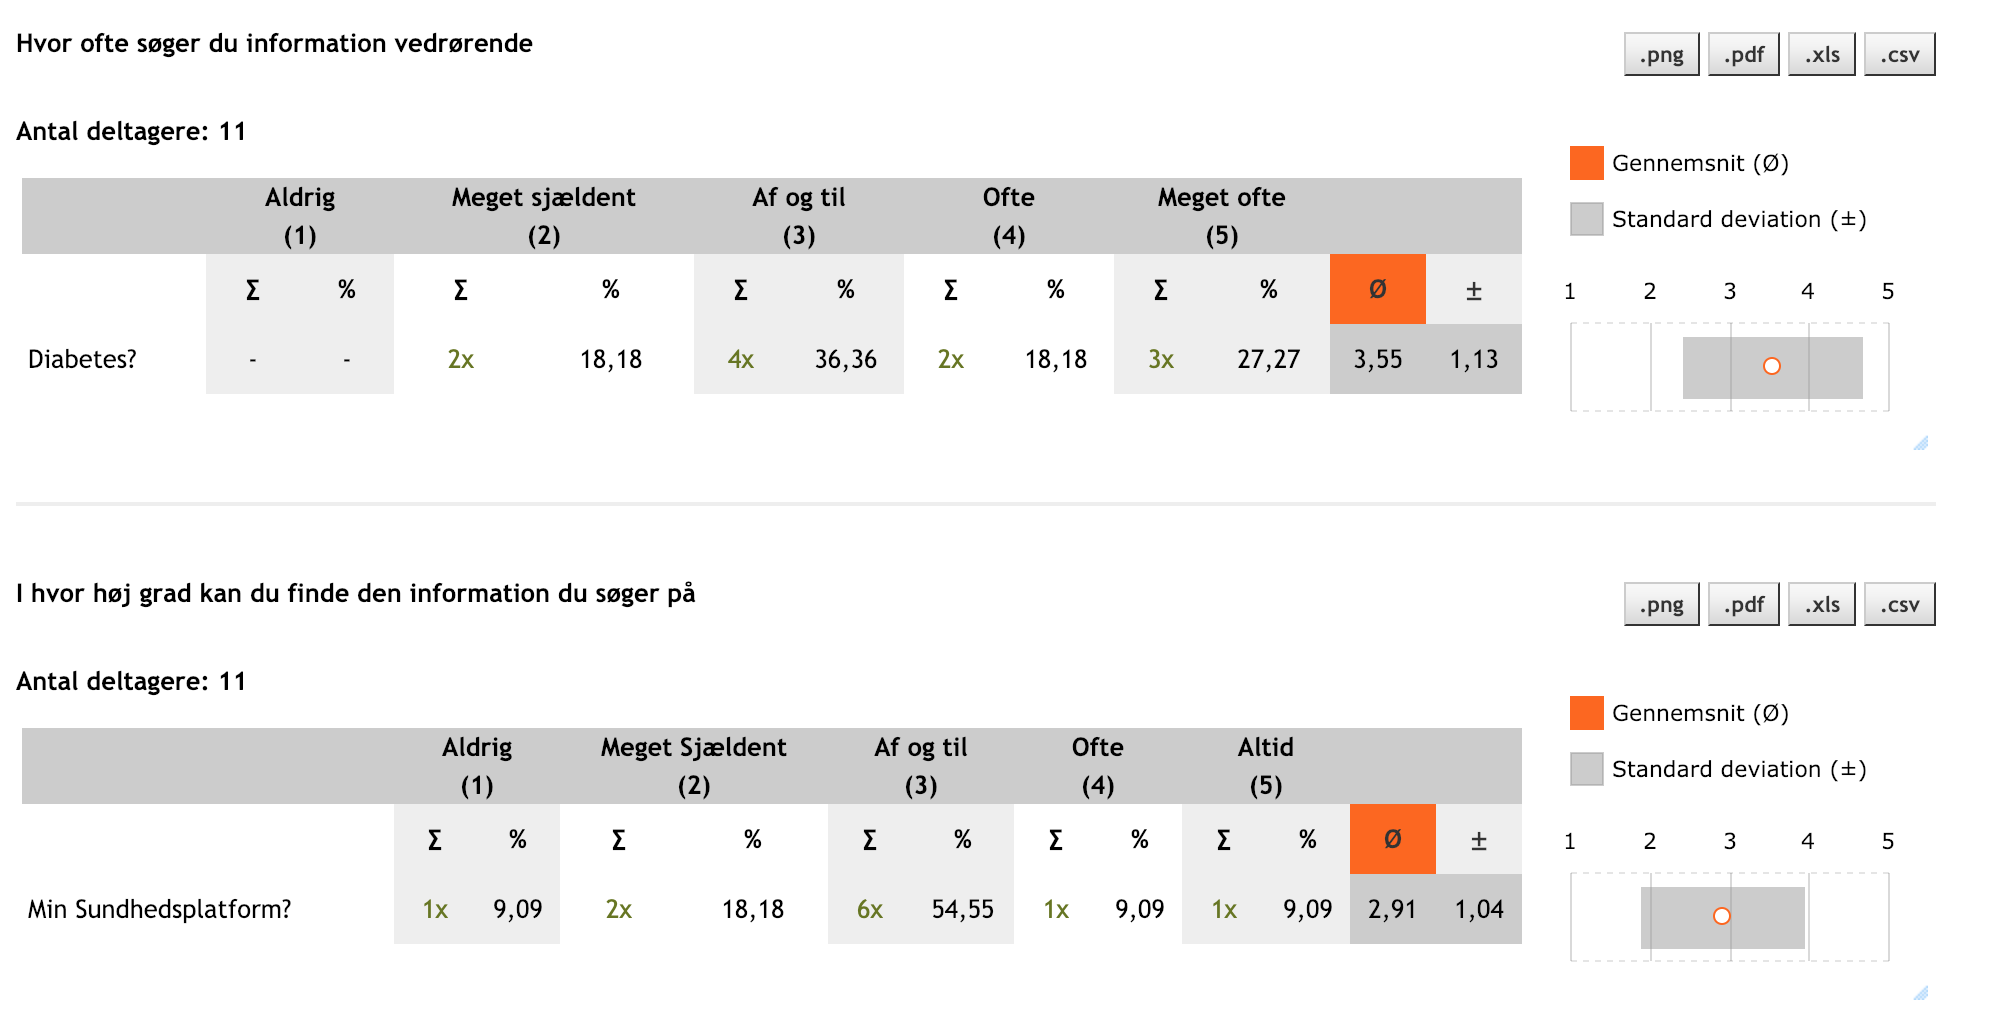
\includegraphics[width=\textwidth]{Materials/SeekingInformation}
	\caption{Svarfordeling på spørgsmål om søgning af information.}
\end{figure}

        	\section{Baggrund og fokus}
Nedenfor ses et sammendrag af vores interviews med vores deltagende diabetes patienter.
\subsection{Interview - Jannie}
Jannie er på førtidspension og har tidligere været pædagog i 8 år. Jannie er normal af bygning, spist almindelig sund kost og altid været sund og rask. Af disse årsager vælger hun i år 2002 at tage forbi Amager Hospital, hvor hun gerne vil melde sig som bloddoner. Dette skal vise sig at være hendes første møde med diabetes på nært hold. Blodprøven viste et højt blodsukkertal og ved senere lægetjek fik hun konstateret diabetes type-2.
\\ \\
I dag tager Jannie medformin 2 gange om dagen og stikker sig med ”insulin-booster” én gang om ugen, hvilket hun beskriver som værende her, at hun for alvor føler at hun er syg. At stikke sig har altid været ubehageligt og sygdomspåmindende i forhold til medformin, som er på tablet-form. Jannie lever som førtidspensionist et meget aktivt liv, hvor hun i ugens løb går til; Yoga mandag, Ipad-kursus tirsdag, synger i gospelkor onsdag, og er frivillig ved hus forbi om torsdagen.
\\ \\
Jannie beskriver sig selv som værende teknisk rutineret, men deltager som førnævnt til Ipad-kursus og vil hele tiden gerne blive klogere på den digitale-verden. Heraf blev dette interview også afholdt via facetime som hun for nyligt var blevet undervist i. Af digitale platforme med relevans for diabetes har Jannie blandt andet benyttet facebook, men har kort inden interviewet afmeldt sig diverse diabetesgrupper, da den løselige information på dette medie ikke sagde hende noget. Herudover benytter hun ”nettet” til informationssøgning – intet specifikt. Jannie har desuden en datter, der læser en sundhedsrelevant uddannelse og får derigennem en masse information vedrørende kost og motion.
\\ \\
Jannie kender ikke til minsp.dk, men er tilknyttet diabetesafdelingen på Amager Hospital, hvor hun kommer ca. hver 3. måned. Her bliver hun vejet, målt, får taget blodprøver og en gang i mellem deltager i lægekonsultation. Hun går desuden også hos egen læge og bestiller tid og recept til hendes medicin igennem lægens eget interne system.
Som afsluttende del af interviewet spurgte vi Jannie om, hvorvidt hun havde en skør idé til en fremtidig digital platform, som kunne hjælpe diabetikere. Et forslag til en ren digital løsning havde hun ikke, men havde som diabetiker ønsket, at hendes sygdomsforløb havde været grebet anderledes an i starten. Hun ville ønske, at der i fremtiden blev sat mere fokus på behandling for nyligt diagnosticerede diabetikere således, at de hurtigt og effektivt kunne blive sat i gang med deres behandling, og at informationsniveauet både var højere og mindre medicinsk anlagt. Hun foreslår, at en personlig vejleder kunne være en mulig løsning (f.eks. en sygeplejeske), der i starten kunne hjælpe én på rette vej – dette kunne evt. sagtens ske via en platform som minsp.dk og via webcam, foreslår hun.

\subsubsection*{Think aloud – minsp.dk}
Jannie logger på minsp.dk på sin Ipad og skal først tilmelde sin e-mail, da det er første gang hun logger på. Herefter tilgår hun de forkellige funktioner på siden. Hun har aldrig været på siden før og  læser op imens hun navigerer rundt: ”Se din 14 seneste tests” siger hun, og trykker sig ind. Hun bliver henrykt over at kunne se sine resulater fra Amager Hospital og oplæser en masse latinske lægefaglige udtryk, som hun ikke forstår og siger ”Hvordan skal jeg på nogen måde kunne forstå disse ting”. Hun navigerer videre på siden og finder hendes andre diagnoser: diabetes type-2, rygsmerter og diskoskolaps. "Ja det passer jo, det har jeg også", siger hun så. Resten af navigationen rundt på siden sker uden problemer, og hun synes, at den virker intuitiv og ret brugervenlig. 

\documentclass[english]{article}
\usepackage[utf8]{inputenc}
\usepackage[T1]{fontenc}
\usepackage{babel}
\usepackage{amsmath}
\usepackage{graphicx}
\usepackage{fancyhdr}
\usepackage{listings}
\usepackage{textcomp}
\usepackage{siunitx}
\usepackage{xcolor}
\usepackage{listings}
\definecolor{commentgreen}{RGB}{2,112,10}
\definecolor{eminence}{RGB}{108,48,130}
\definecolor{weborange}{RGB}{255,165,0}
\definecolor{frenchplum}{RGB}{129,20,83}
\lstset {
    language=python,
    frame=tb,
    tabsize=4,
    showstringspaces=false,
    numbers=left,
    upquote=true,
    commentstyle=\color{commentgreen},
    keywordstyle=\color{eminence},
    stringstyle=\color{red},
    basicstyle=\small\ttfamily, % basic font setting
    emph={int,char,double,float,unsigned,void,bool},
    emphstyle={\color{blue}},
    escapechar=\&,
    % keyword highlighting
    classoffset=1, % starting new class
    morekeywords={>,<,.,;,,,-,!,=,~},
    keywordstyle=\color{weborange},
    classoffset=0,
}
\pagestyle{fancy}
\fancyhf{}
\renewcommand{\headrulewidth}{0pt}
\setlength{\headheight}{0pt} 

\begin{document}

\section*{Interview - Ernst}
Ernst er type-2 diabetiker og arbejder til dagligt som buschauffør. Ernst fik konstateret diabetes tilbage i år 2005, hvor han som bloddoner fik en melding om alt for højt blodtryk. Derfor kom han  til kontrol hos egen læge, hvor han herefter fik sin diagnose.
I starten gik han til egen læge hver 3. måned og fik medformin, som er tablet-medicin for diabetikere. I starten tog Ernst meget let på sin sygdom og de første mange år gik han uden at ændre sin livsstil. Ernst led af stor overvægt og dårlige madvaner – heraf fortalte Ernst at han især var glad for ostemader, hvor 10 stk. dagligt ikke var helt ualmindeligt.
Omkring år 2015 får Ernst beskeden om at han skal være bedstefar, dette var en stor øjenåbner for ham og et opråb om at en livsstilsændring skulle til for at hans levealder og tid sammen med barnetbarnet kunne forlænges. Hans startede derfor hvor det stod værst til – ved hans livstil.
\\ \\
Ernst vælger at tilmelde sig TV2 programmet “Kan man spise sig rask”, hvor han bliver castet, deltager og opnår flotte resultater. Siden har han taget en Umahro-uddannelse (Sundhedsrådgiver) og hjælper ligesindede ved at brede sit budskab vedr. diabetes, og hvordan man kan behandle sin sygdom på andre områder end via de medicinske veje, som han oplever har været omdrejningspunktet i de lægefaglige kræse – hvilket han har en meget stærk holdning til. Herudover er Ernst tilknyttet frivilligcenteret i kommunen, hvor han fortæller og vejleder i KRAM-faktorene (Kost, rygning, alkohol og motion)
\\ \\
Ernst kender ikke til minsundhedsplatform.dk, men er dog tilknyttet Nykøbing Falster Sygehus, hvor han deltager i årlig kontrol. Muligheden for mindst én kontrol årligt som diabetiker blev han først opmærksom på efter, at have været hos egen læge i flere år og har tidligere haft dårlige erfaringer med sin egen læge og dertilhørende henvisninger til informative og støttende foreninger for diabetikere. Det var først da Ernst, fik sit barnebarn at han vendte op og ned på sit liv. 
\\ \\
Ernst er som tidligere nævnt tilknyttet Sygehuset i Nykøbing på Lolland Falster, hvor han årligt går til kontrol. Han mener at fagpersonalet har valgt at sende ham e-mails med de prøvesvar og kontroller han har gået til, men har tilsyndeladende ikke tjekket op på dette et stykke tid, da han ikke rigtigt kan huske det. Han mener at han stadigvæk får e-mails tilsendt, og har hvertfald ikke været opmærksom på minsp.dk. Ernst foretrækker personlig kontakt, hvorfor han i dag også fornyer sin recept via telefon og ikke via lægens interne systemer. Af andre digitale platforme benytter Ernst facebook, hvor han fortæller og rådgiver andre diabetikere med sine egne erfaringer, men er samtidig også skeptik og afholdende fra at modtage gode råd fra disse grupper.
\\ \\
Generelt er Ernst utilfreds med den måde, hvorpå hospitalsvæsenet håndterer diabetes idet, at han får for lidt information omkring alternativ sygdomsbekæmpelse end den medicinske. Han mener at det er økonomiske årsager mellem det offentlige og medicinindustrien der spiller en væsentlig rolle for denne behandlingsmetode. Han fortæller at han var underinformeret omkring blandt andet aflæsning af tal og hvordan han skulle gribe sin livsstilsændring an igennem mange år af sit sygdomsforløb. Ernst savnede især “gode eksempler” hvilket han foreslå for eksempel kunne komme via video på nettet. Overordnet har Ernst manglet motivation og information omkring hvor og hvordan han kunne blive klogere på metoder til at takle sin dagligdag fra den dag han fik konstateret diabetes.

\subsection*{Think aloud – minsp.dk} 
Ernst loggede på minsp.dk via hans computer og fandt platformen ret intuitivt. Her kunne Ernst tilgå de forskellige funktioner på siden uden problemer og viste stor interesse og nysgerrighed om denne side han ikke før havde hørt om. Han kiggede på nogle tidligere journaler, men var dog i tvivl om nogle af de aktuelle journalers indhold, om hvorfra og hvilken kontrol disse stammede fra. Han havde ikke yderligere kommentarer til siden som helhed og indtrykket var overordnet positivt.



\end{document}
\subsection{Interview - Karen}
Karen er pensioneret sekretær og fik konstateret type-2 diabetes i en ret ung alder. I starten fortalte hun at hun var meget underinformeret, hvor hun var bange for sin sygdoms konsekvenser og ikke vidste hvordan hun skulle håndtere sin sygdom. Dette fik hende til at spise utrolige mængder rugbrød uden pålæg som et desperat forsøg på at komme hendes sygdom til livs, hvilket resulterede i at hun tog meget på i vægt i den periode. Hun mente at informationsniveauet i starten var utilstrækkelig og manglede generelt information til hvordan hun skulle gribe sin sygdom an i forhold til fremtidig bahandling. I dag tager hun medformin, 2 piller morgen og aften, og lever et godt og aktivt liv trods sin sygdom.
\\ \\
Karen har tidligere været tilknyttet Bispebjerg sygehus, hvor hun blandt andet har deltaget i projekter og forløb vedrørende hendes sygdom. Hvordan hun i sin tid fik svar og resultater fra disse kontroller og forsøg kunne hun ikke huske, da det var lang tid siden. Karen er i dag ikke tilknyttet et sygehus, men kender dog til minsp.dk, hvor hun en enkelt gang eller to har læst prøvesvar vedr. Hendes sukkertal, som hun mener hendes læge indtaster, men det var hun desværre ikke klar over. 
\\ \\
Hun har generelt ikke benyttet minsp.dk meget, men kun været nysgerrig på hvad det var. Hun har herudover også downloaded app'en, som hun synes er meget brugervenlig i udseende, men bruger den ikke overhovedet. Hun finder minsp.dk brugervenlig og kan i det hele taget godt lide at benytte digitale platforme, hvilket også betyder hun fornyer recept hos egen læge digitalt, via læges eget interne system. Hun går til kontrol ved egen læge hver 3 mdr. Hun synes at det er ægerligt at der ikke findes et samlingssted for diabetikere online, hvor mange ting er samlet under ét hvor man kan få den fornødne information man har behov for. En kommentar vedr. mållinger var at der bliver benyttet forskellige talbetegnelser for blodsukkeret, blandt fagfolk, digitale målemaskiner o.lign, hvilket hun fandt ret frustrerende, og at det var hende selv som skulle finde information og omregne tal. 
Som en afsluttende del af interviewet bad vi Karen foreslå en skør idé til et digitalt produkt/platform som kunne hjælpe diabetikere i hendes øjne. Karens forslag var et mere specificeret samlingssted for diabetikere, hvor der var mere håndgribelig information til især ny-diagnosticerede patienter.
\\ \\
Karen sidder tilligemed i en styregruppe, hvor hun som brugerrepræsentant for diabetikere kommer med indput til omlægning eller tilknytning af anden telefonlinje til diabetikere istedet for 1813, så man akut kan få hjælp af fagspecialister i diabetes 24 timer i døgnet.

\subsubsection*{Think aloud - minsp.dk}
Karen har benyttet minsp.dk til at tjekke prøvesvar og blodsukkertal før, men er ikke jævnlig bruger af platformen. Hun finder siden brugervenlig og har benyttet den under dette interview, men var generelt meget kortfattet omkring hendes oplevelser under brugen af siden. Under think-aloud-testen navigerede Karen rundt på siden, hvor hun gennemgik forskellige funktionaliteter på hjemmesiden under vores forespørgsel, heriblandt: Kontakt til hospital/læge, aktuelle diagnoser og prøvetal, journal samt information vedr. Sygdom. Dette klarede Karen uden nogle problemer og hun virkede generelt til at være en rutineret bruger af digitale platforme og fandt hurtigt frem til de punkter som fremlagt under denne test. En bemærkelse var dog at Karen under testen havde lidt problemer med at tilgå "receptfornyelse samt booking/aftaler" som lå under samme menupunkter, om det skyldes et internetproblem eller selve siden er uvist, men hun virkede til at være teknisk i stand til at finde disse punkter. 
\\ \\
Overordnet set var hendes opfattelse af siden var ret positiv og at den fremkom brugervenlig og at det generelt var et overskueligt system set fra et interaktivt synspunkt, men syntes at det var svært at forstå tal og prøvesvar generelt og kunne godt have brug for bedre vejledning til hendes tidligere prøvesvar.

\subsection{Interview - Morten}
Morten er 41 år og fik for ca. 8-10 år siden konstateret diabetes type-2. Morten havde gået syg i en længere periode (konstant været snottet, følt sig skidt tilpas og tabt sig mange kg.). Derfor tager han til sin egen læge. Hos lægen får Morten konstateret diabetes type-2 og målt et alt for højt blodsukkerniveau.
\\ \\
Morten er tilknyttet egen læge, hvor han går til personlig konsultation og får målt sit blodsukker. Han går hos sin læge ca. hver 3 måned og fornyer sin recept via lægens interne system som han finder nemt og ligetil, og han foretrækker elektronisk bestilling. Morten er ikke tilknyttet et hospital, men er dog bekendt med minsp.dk, hvor han går ind og tjekker sine blodsukkertal, vitaminmangel, kolesteroltaltal og andre målinger som hans egen læge har indtastet. Morten kender ikke til app'en, men er positiv over at sådan en findes og vil efter egen udsagn formentligt benytte platformen oftere end hjemmesiden. 
\\ \\
Morten synes ikke han mangler noget vedrørende hans sygdom. Hans kone er sygeplejeske og han får derigennem en masse information vedrørende diabetes. Han fortæller dog at han i starten af sin sygdom manglede en masse information og at det først var for nyligt at han han havde fået et gennembrud med en alternativ behandlingsform end den medicinske vej. Ifølge ham selv er der alt for lidt fokus på alternativ behandling og han har derfor i samråd med hans kone fulgt et low-carp kost-program og omlagt sine kostvaner drastisk, hvilket har resulteret i, at han i dag har lagt ”medformin” på hylden som han ellers har taget fast i ca. 9 år. Det betyder at Morten i dag ikke tager medicin overhovedet – med stor succes. Han forslår et digitalt samlingssted for diabetikere, hvor man kan få rådgivning om selv de mindste kostråd, så folk kommer væk fra ”løs” informationssøgning på facebook og diverse internet-sider online. 

\subsubsection*{Think aloud – minsp.dk}
Morten kender godt til minsp.dk og benytter den en gang imellem, men ikke mere end de besøg han har haft hos lægen. Morten var kort af ord og vi prøvede ikke at tilgå siden sammen, men han kommenterede på sine oplevelser af siden alligevel. Han fandt ikke siden besværlig at navigere rundt på, men kommenterede at siden hvertfald ikke var mobiloptimeret, hvilket han synes være lidt irriterende når han skulle bruge den. De resterende funktionaliteter som forefindes på hjemmesiden benytter han ikke.

\subsection{Fokuspunkter}
\subsubsection{Et sted med al information (info om sygdom, kost, prøve-svar mm.)}
Alle vores interviewpersoner har det tilfælles, at de har været informationssøgende på egen hånd langt hen af vejen, og vi oplever derfor et stort område, hvor der er plads til forbedring. I tilkobling til minsp.dk og patienters rutinetjek hos fagfolk, bør information vedr. deres individuelle behandling være samlet ét sted.

\subsubsection{En mere personlig Min Sundhedsplatform}
Diabetes er en velkendt sygdom, hvor store dele af behandlingen er kendt på forhånd. Derfor bør det være muligt at tilbyde patienter personlig kontakt med f.eks. studerende eller sygeplejersker, der kan give almene råd om f.eks. alternativ behandling, støtte og overordnet hjælp til dem, som ønsker.

\subsubsection{Brugervenlighed af Min Sundhedsplatform}
Brugen af Min Sundhedsplatform er varierende blandt vores interviewdeltagere. Nogle benytter flittigt siden, mens andre sjældent eller aldrig benytter den. For at få et indblik i hvor intuitiv og brugervenlig siden er, udførte vi en think aloud test sammen med vores deltagere. Her bad vi dem finde aktuelle diagnoser, journaler, forny deres recept, finde prøvesvar, booke en aftale med egen læge eller hospital, finde et link til 'patienthaandbogen.dk' og finde et link til 'sundhed.dk'. Overordnet fandt alle siden intuitiv og nem at navigere. Jannie som ikke var en hyppig bruger af siden blev begejstret for den information hun kunne finde, men samtidig fandt hun det besværligt at tolke på den information som hun kunne finde. For eksempel finder hun det svært at tolke sine prøvesvar. Ligeledes finder Karen det svært at tolke prøvesvar. Hun fortæller at forskellige sider benytter forskellige enheder til prøver, og at hun selv må omregne sine prøvesvar.\\
Morten og Julia fortæller, at mobilsiden ikke fungerer optimalt, og der kunne gøres store forbedringer der.\\
Overordnet finder vores deltagere siden, uanset om de har benyttet den før eller ej, intuitiv og brugervenlig, og de fleste kunne løse alle vores stillede opgaver.

\subsubsection{Motivation}
En væsentlig og direkte stærk behandling af diabetes kræver ofte en drastisk livsstilsændring, hvilket for mange kan være en stor omvæltning af dagligdagen og dårlige vaner. Dette kan sidestilles med personer som gennemgår et rygestop. Som led i dette kan motivation være en vigtig faktor for at gennemføre sådanne ændringer, hvorfor en både nem og let implementerbar løsning kunne være videomateriale med "gode eksempler" fra folk, der har opnået succes med f.eks alternativ behandling.

\subsubsection{Alternativ behandling}
Ernst følte ikke at han fik tilstrækkelig information omkring alternativer til hans behandling. Efter ikke at have taget sin sygdom synderligt seriøst i en længere periode, fik han et barnebarn og blev klar over, at han var nødt til at lægge sit liv om. Han oplever dog stadig ikke, at den 'medicinske vej' er den rigtige måde at håndtere sin sygdom på. Ernst og Morten er de eneste, som benytter alternativ behandling, hvilket kan skyldes, at diabetikere bliver underinformeret omkring dette, eller at størstedelen af diabetikere foretrækker den kliniske behandling. 

\subsubsection{Uniforme prøvesvar}
Flere af interviews personer oplever at deres prøvesvar er svære at forstå og de er i tvivl om betydningen af prøvesvarende. De savner mere uddybende forklaring og mere gense navne til prøvesvarene. 
Der var flere at prøvesvarende interviews personer ikke viste hvad var fordi de ikke forstod de latinske lægefaglige udtryk.\\
Interviews personer ønsker også at der stod hvor / hvilken hospital prøvesvarene var blevet taget.

\subsubsection{Overflod af fagtermer}
I vores interview med Jannie fik vi hende til at tilgå sine prøvesvar, hvilket hun ikke har gjort før på MSP. Omend hun først var henrykt over at kunne se sine prøvesvar, så blev hun meget skuffet da hun ikke kunne forstå dem, idet de tekniske detaljer var mange og ikke var præsenteret på en form, som var forståelig for det almene individ men i stedet henvendte sig til fagteknisk personale. Færre medicinske betegnelser til fordel for et mere forståeligt sprog ville være at foretrække. 

\subsubsection{Receptfornyelse-påmindelse}
Cirka halvdelen af interviews personer fortrækker at fornyer deres recept via personlig kontakt til egen læge f.eks. via telefon. Den anden halvdelen fornyer deres recept digitalt, men via egen læges interne digitale system eller via sundhed.dk. \\
Det er i dag mulig at lave recept fornyelse via Min Sundhedsplatform ved at sende en mail til hospitalet. Et mål kunne være at flytte måden man receptfornyer over i Min Sundhedsplatform.

\subsubsection{Skabe opmærksomhed omkring Min Sundhedsplatform}
Et gennemgående tema på tværs af vores interviews, har været, at der er manglende kendskab til Min Sundhedsplatform. Selv kronisk syge diabetikere har manglende kendskab til denne side, på trods af at være et stort initiativ fra regionens side til at simplificere kontakt mellem patient og læge. Derfor ville en kampagne for at skabe yderligere kendskab til MSP blandt beboerne i Region Hovedstaden/Sjælland være gavnligt.

\subsubsection{Diskussionsforum for patienter}
I vores samtale med Morten konkluderede vi, at der var et afsavn på diverse diskussionsfora for diabetikere, hvor information omkring diabetes kunne deles blandt de pårørende.
Dog konkluderede vi ligeså i vores samtale med Ernst, at der er en vis skeptisk overfor information, som modtages igennem sådanne fora. En god mellemløsning mellem disse to problemstillinger kunne være at implementere et diskussionsforum på Min Sundhedsplatform, hvor man som patient kan stille og søge på spørgsmål, som læger/sygeplejersker/andre sundhedsfagligt personale kunne besvare, således at der er yderligere tiltro samt kvalitet bag disse svar, som almene patienter har mulighed for at stille. 


        	\section{Konsekvensanalyse}
I vores arbejde har vi henvendt os til otte hospitaler, lægepraksisser og diætister, men vores henvendelse er desværre enten blevet ignoreret, eller stedet har ikke haft tid til at have os på besøg. Vi har derfor skrevet en konsekvensanalyse over konsekvenserne af, at vi ikke har været i kontakt med sundhedsfagligt personale under denne fase.
 
\begin{adjustbox}{angle=90}
	\begin{tabularx}{0.81\textheight}{|>{\columncolor{WhiteGray}}X|>{\columncolor{LightGray}}X|>{\columncolor{WhiteGray}}X|>{\columncolor{LightGray}}X|>{\columncolor{WhiteGray}}X|}
		\hline
		\rowcolor{Gray}
		\textbf{Situationer som skaber pres} & \textbf{Konsekvenser} & \textbf{Forebyggende tiltag} & \textbf{Afhjælpende tiltag} & \textbf{Relevante samarbejdspartnere}\\
		\hline
		Ingen mulighed for at opleve arbejdspraksis på hospitaler, praktiserende læger, diætist mf.
		&Forlænget arbejdsopgave. (Produktet kræver flere iterationer når behov og krav ikke er tænkt ind fra start).
		&
		&Sende billeder til sundhedsfagligt personale tidligt i processen med udarbejdelse af prototype og få feedback.
		&Patienter.\\[100pt]
		\hline
		&Manglende forståelse for behov og krav.
		&
		&Kontakt sundhedspersonale under uddannelse / næsten færdig med uddannelse.
		&Lægestuderende.\\[100pt]
		\hline
		&Manglende indblik i arbejdspladsens teknologiske forståelse.
		&
		&Bede om skriftlig beskrivelse af forhold, arbejdsopgaver, ønsker mm.&\\[100pt]
		\hline
		&Manglende forståelse for tiden til hver opgave og stress.&&&\\[0.2\textwidth]
		\hline
	\end{tabularx}
\end{adjustbox}

        	\section{ER Diagram}
\begin{figure}[H]
  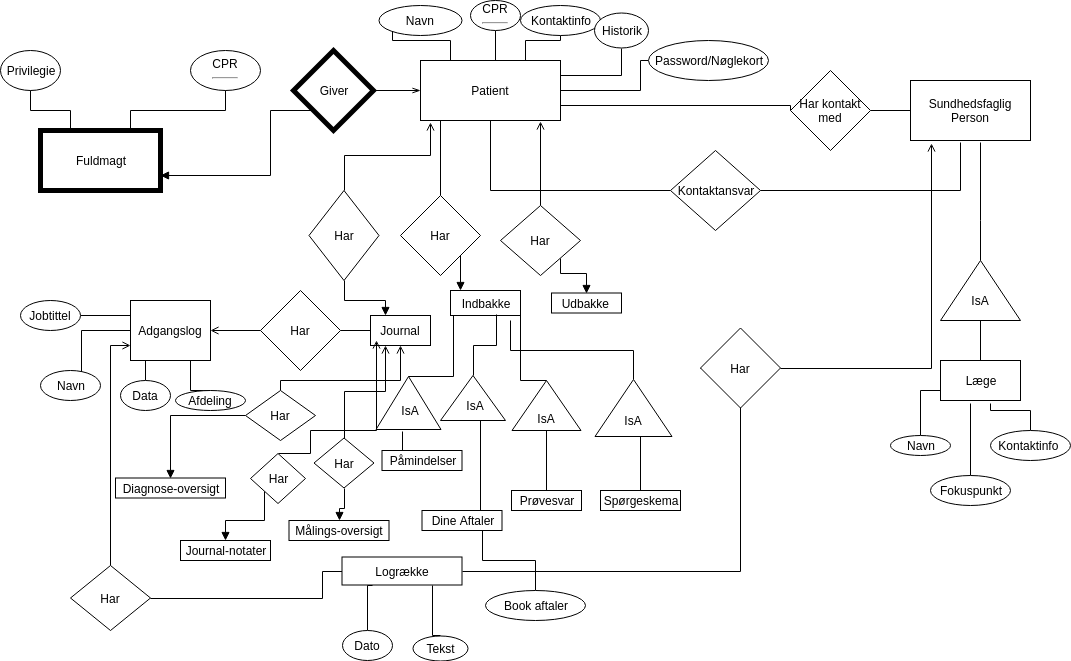
\includegraphics[width=\linewidth]{Materials/ER-diagram.png}
  \caption{ER-diagram for Min Sundhedsplatform}
  \label{fig:ER}
\end{figure}
ER Diagrammet (Ovenstående figur \ref{fig:ER}) viser den logiske model for domænet Min Sundhedsplatform. \\
Entiteterne er de logiske enheder - dvs. aktører, objekter og begivenheder i systemet. 
Relationerne angiver hvilken type af relation, der er mellem entiteterne i systemmet.

Entiteterne angives med rektangler og en tekst typisk et navneord. Til entiteterne er der tilknyttet et eller flere attributter, angivet med en ellipse med en tekst.

Relationerne angives med en diamant med en  tekst, der beskriver relationen mellem to eller flere entiteter.

kardinaliteten beskrives med streger og pile mellem entiteterne. \\ 
En sort lukket pil beskriver: mange til højst en (dvs. 0 eller 1).\\
En åben pil beskriver: mange til præcis en.\\
En streg uden pil beskriver: mange til mange.

Under-entiteter repræsenteres med relationen 'ISA' i en trekant.

En svag entitet er en entitet, der for at relationen kan gælde, kræver at den udover sine egne attributter også skal have sin ejers nøgleattribut som nøgle. Den beskrives med en fed ramme.

Vi kan læse følgende information om Min Sundhedsplatform ud af ER Diagrammet:\\
En patient har tilknyttet attributterne: navn, cpr-nummer, kontakt-info, historik og password/nøglekort. Cpr-nummer er nøgleattribut.\\
Der er en giver-relation fra entiteten patient til entiteten fuldmagt. Der er en mange til en relation, fordi patienten giver fuldmagter og fuldmagterne er givet af én patient. Fuldmagt er en svag entitet, fordi den kræver sin ejers nøgleattribut - dvs. patientens cpr-nummer som nøgleattribut. \\
Patienter har kontakt med mange sundhedsfaglige personer og mange  sundhedsfaglige personer har kontakt ansvar med mange patienter. Læger er under-entitet af sundhedsfaglig personale. \\
Patienten har højest én udbakke, og udbakken tilhører præcis en patient.\\
Patienten har højest én indbakke. Indbakke kan være Påmindelser, Dine Aftaler, Prøvesvar og Spørgeskema.\\
Patienten har højest én journal og en journal tilhører præcis en patient. \\
Journalen har præcis én adgangslog, som har mange logrækker. Logrækken har præcis en adgangslog og præcis en sundhedsfaglig person. En sundhedsfaglig person har mange logrækker.\\
Journalen har én eller ingen diagnose-oversigt og diagnose oversigten tilhører præcis en journal.\\
Journalen har enten ingen eller en journal-notater som tilhører præcis én journal.\\
Journalen har enten én eller ingen målings-oversigt som tilhører præcis én journal.

I designfasen kan den logiske model af ER diagrammet bruges til at danne et overblik over hvilke data, der skal gemmes i systemet, og hvordan flowet er (relationerne mellem entiteterne).\\
ER-diagrammet kan bruges i kommunikationen mellem it-designeren, kunden og brugerne omkring afklaringen af hvilke data, der skal indgå i systemet/domænet. \\
I udviklingsfasen kan ER-diagrammet transformeres til den fysiske model hvor man, ud fra entiteterne, opstiller databaserne/tabeller med de attributter/data, der er behov for i domænet.

        \end{document}
